\documentclass[tikz, border=10pt]{standalone}
\usepackage{pgfplots}
\pgfplotsset{compat=1.18}
\usetikzlibrary{fillbetween}

\begin{document}
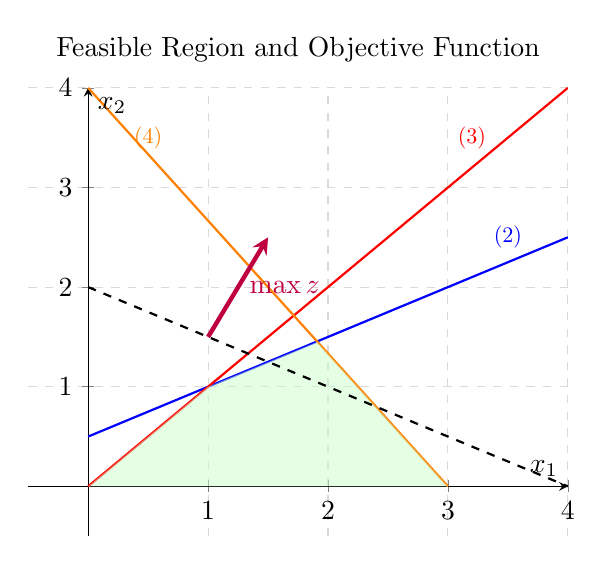
\begin{tikzpicture}
    \begin{axis}[
        axis lines = middle,
        xlabel = {$x_1$},
        ylabel = {$x_2$},
        xmin = -0.5, xmax = 4,
        ymin = -0.5, ymax = 4,
        grid = both,
        grid style = {dashed, gray!30},
        title = {Feasible Region and Objective Function}
    ]

    % Define the constraint lines
    \addplot[name path=C1, blue, thick, domain=0:4] {0.5*x + 0.5}; % -x1 + 2x2 = 1
    \addplot[name path=C2, red, thick, domain=0:4] {x};            % -x1 + x2 = 0
    \addplot[name path=C3, orange, thick, domain=0:3] {4 - (4/3)*x}; % 4x1 + 3x2 = 12
    \addplot[name path=Axis, draw=none, domain=0:3] {0};          % x-axis

    % Fill the feasible region
    % The vertices are (0,0), (1,1), (1.91, 1.45), (3,0)
    \fill[green!20, opacity=0.5] (axis cs:0,0) -- (axis cs:1,1) -- (axis cs:1.91, 1.45) -- (axis cs:3,0) -- cycle;

    % Highlight the objective function gradient/direction (max x1 + 2x2)
    % Showing a level curve x1 + 2x2 = 4 (e.g., x2 = 2 - 0.5x1)
    \addplot[dashed, black, thick, domain=0:4] {2 - 0.5*x};
    \draw[->, >=stealth, ultra thick, purple] (axis cs:1, 1.5) -- (axis cs:1.5, 2.5) 
        node[midway, right] {$\max z$};

    % Labels for constraints
    \node[blue, scale=0.8] at (axis cs:3.5, 2.5) {(2)};
    \node[red, scale=0.8] at (axis cs:3.2, 3.5) {(3)};
    \node[orange, scale=0.8] at (axis cs:0.5, 3.5) {(4)};

    \end{axis}
\end{tikzpicture}
\end{document}